% Options for packages loaded elsewhere
% Options for packages loaded elsewhere
\PassOptionsToPackage{unicode}{hyperref}
\PassOptionsToPackage{hyphens}{url}
\PassOptionsToPackage{dvipsnames,svgnames,x11names}{xcolor}
%
\documentclass[
  letterpaper,
  DIV=11,
  numbers=noendperiod]{scrartcl}
\usepackage{xcolor}
\usepackage{amsmath,amssymb}
\setcounter{secnumdepth}{-\maxdimen} % remove section numbering
\usepackage{iftex}
\ifPDFTeX
  \usepackage[T1]{fontenc}
  \usepackage[utf8]{inputenc}
  \usepackage{textcomp} % provide euro and other symbols
\else % if luatex or xetex
  \usepackage{unicode-math} % this also loads fontspec
  \defaultfontfeatures{Scale=MatchLowercase}
  \defaultfontfeatures[\rmfamily]{Ligatures=TeX,Scale=1}
\fi
\usepackage{lmodern}
\ifPDFTeX\else
  % xetex/luatex font selection
\fi
% Use upquote if available, for straight quotes in verbatim environments
\IfFileExists{upquote.sty}{\usepackage{upquote}}{}
\IfFileExists{microtype.sty}{% use microtype if available
  \usepackage[]{microtype}
  \UseMicrotypeSet[protrusion]{basicmath} % disable protrusion for tt fonts
}{}
\makeatletter
\@ifundefined{KOMAClassName}{% if non-KOMA class
  \IfFileExists{parskip.sty}{%
    \usepackage{parskip}
  }{% else
    \setlength{\parindent}{0pt}
    \setlength{\parskip}{6pt plus 2pt minus 1pt}}
}{% if KOMA class
  \KOMAoptions{parskip=half}}
\makeatother
% Make \paragraph and \subparagraph free-standing
\makeatletter
\ifx\paragraph\undefined\else
  \let\oldparagraph\paragraph
  \renewcommand{\paragraph}{
    \@ifstar
      \xxxParagraphStar
      \xxxParagraphNoStar
  }
  \newcommand{\xxxParagraphStar}[1]{\oldparagraph*{#1}\mbox{}}
  \newcommand{\xxxParagraphNoStar}[1]{\oldparagraph{#1}\mbox{}}
\fi
\ifx\subparagraph\undefined\else
  \let\oldsubparagraph\subparagraph
  \renewcommand{\subparagraph}{
    \@ifstar
      \xxxSubParagraphStar
      \xxxSubParagraphNoStar
  }
  \newcommand{\xxxSubParagraphStar}[1]{\oldsubparagraph*{#1}\mbox{}}
  \newcommand{\xxxSubParagraphNoStar}[1]{\oldsubparagraph{#1}\mbox{}}
\fi
\makeatother


\usepackage{longtable,booktabs,array}
\usepackage{calc} % for calculating minipage widths
% Correct order of tables after \paragraph or \subparagraph
\usepackage{etoolbox}
\makeatletter
\patchcmd\longtable{\par}{\if@noskipsec\mbox{}\fi\par}{}{}
\makeatother
% Allow footnotes in longtable head/foot
\IfFileExists{footnotehyper.sty}{\usepackage{footnotehyper}}{\usepackage{footnote}}
\makesavenoteenv{longtable}
\usepackage{graphicx}
\makeatletter
\newsavebox\pandoc@box
\newcommand*\pandocbounded[1]{% scales image to fit in text height/width
  \sbox\pandoc@box{#1}%
  \Gscale@div\@tempa{\textheight}{\dimexpr\ht\pandoc@box+\dp\pandoc@box\relax}%
  \Gscale@div\@tempb{\linewidth}{\wd\pandoc@box}%
  \ifdim\@tempb\p@<\@tempa\p@\let\@tempa\@tempb\fi% select the smaller of both
  \ifdim\@tempa\p@<\p@\scalebox{\@tempa}{\usebox\pandoc@box}%
  \else\usebox{\pandoc@box}%
  \fi%
}
% Set default figure placement to htbp
\def\fps@figure{htbp}
\makeatother





\setlength{\emergencystretch}{3em} % prevent overfull lines

\providecommand{\tightlist}{%
  \setlength{\itemsep}{0pt}\setlength{\parskip}{0pt}}



 


\KOMAoption{captions}{tableheading}
\makeatletter
\@ifpackageloaded{caption}{}{\usepackage{caption}}
\AtBeginDocument{%
\ifdefined\contentsname
  \renewcommand*\contentsname{Table of contents}
\else
  \newcommand\contentsname{Table of contents}
\fi
\ifdefined\listfigurename
  \renewcommand*\listfigurename{List of Figures}
\else
  \newcommand\listfigurename{List of Figures}
\fi
\ifdefined\listtablename
  \renewcommand*\listtablename{List of Tables}
\else
  \newcommand\listtablename{List of Tables}
\fi
\ifdefined\figurename
  \renewcommand*\figurename{Figure}
\else
  \newcommand\figurename{Figure}
\fi
\ifdefined\tablename
  \renewcommand*\tablename{Table}
\else
  \newcommand\tablename{Table}
\fi
}
\@ifpackageloaded{float}{}{\usepackage{float}}
\floatstyle{ruled}
\@ifundefined{c@chapter}{\newfloat{codelisting}{h}{lop}}{\newfloat{codelisting}{h}{lop}[chapter]}
\floatname{codelisting}{Listing}
\newcommand*\listoflistings{\listof{codelisting}{List of Listings}}
\makeatother
\makeatletter
\makeatother
\makeatletter
\@ifpackageloaded{caption}{}{\usepackage{caption}}
\@ifpackageloaded{subcaption}{}{\usepackage{subcaption}}
\makeatother
\usepackage{bookmark}
\IfFileExists{xurl.sty}{\usepackage{xurl}}{} % add URL line breaks if available
\urlstyle{same}
\hypersetup{
  pdftitle={Mes Projets},
  colorlinks=true,
  linkcolor={blue},
  filecolor={Maroon},
  citecolor={Blue},
  urlcolor={Blue},
  pdfcreator={LaTeX via pandoc}}


\title{Mes Projets}
\author{}
\date{}
\begin{document}
\maketitle

\renewcommand*\contentsname{Table of contents}
{
\hypersetup{linkcolor=}
\setcounter{tocdepth}{3}
\tableofcontents
}

\section{🚀 Projets en Data Science \& Développement
IA}\label{projets-en-data-science-duxe9veloppement-ia}

\subsection{\texorpdfstring{📊
\href{https://github.com/dona-eric/Hack2Hiere_TechTech_DataScience_20}{Hack2Hiere
Tech DataScience
2020}}{📊 Hack2Hiere Tech DataScience 2020}}\label{hack2hiere-tech-datascience-2020}

\begin{figure}[H]

{\centering \pandocbounded{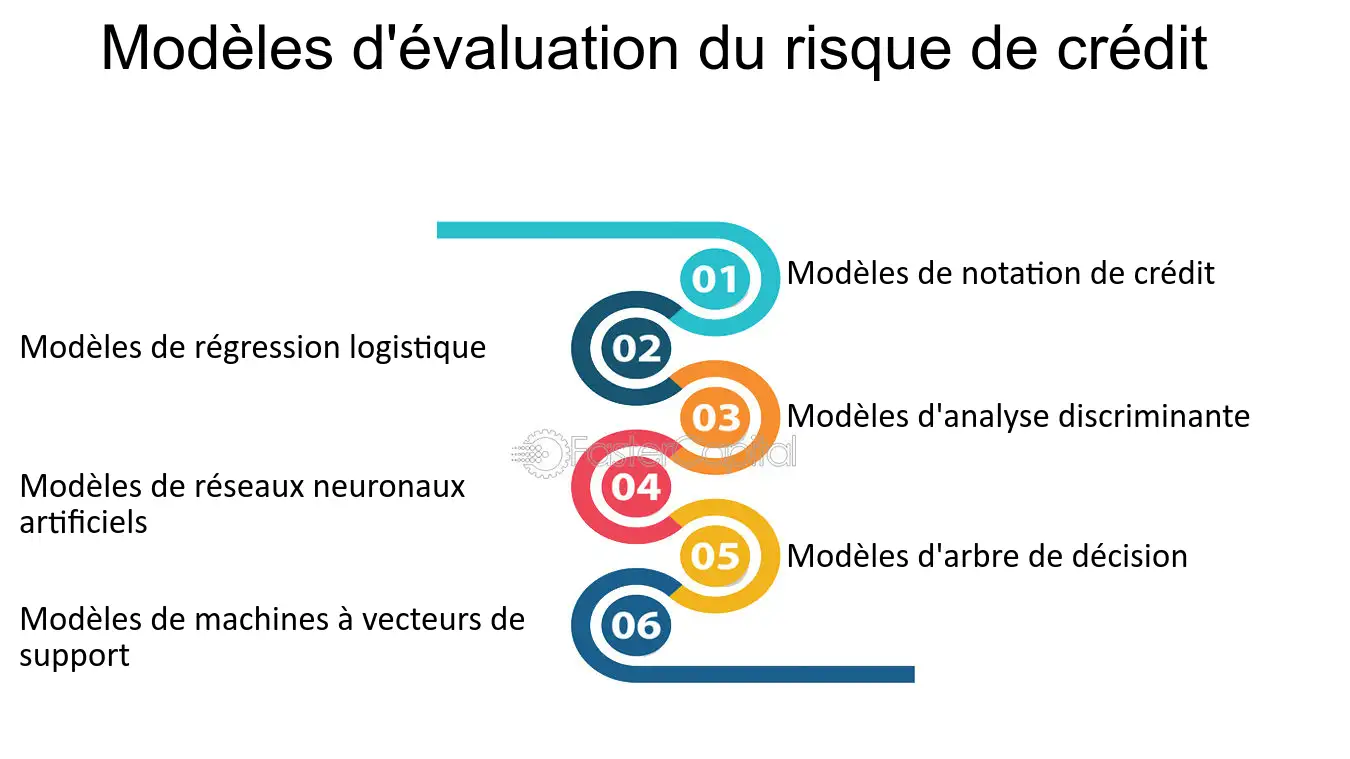
\includegraphics[keepaspectratio]{images/hack-tech.jpg}}

}

\caption{Hack2Hiere}

\end{figure}%

Exploration des données pour identifier les principales variables
corrélées à l'octroi de crédit. Développement d'un modèle de scoring
crédit permettant de prédire la probabilité d'octroi.

📌 \textbf{Stack} : Pandas, Scikit-learn, Matplotlib, classification
supervisée.

\begin{center}\rule{0.5\linewidth}{0.5pt}\end{center}

\subsection{\texorpdfstring{😄
\href{https://github.com/dona-erick/Projet-Reconnaissance-Emotion-RealTime}{Système
de Reconnaissance d'Émotions en Temps
Réel}}{😄 Système de Reconnaissance d'Émotions en Temps Réel}}\label{systuxe8me-de-reconnaissance-duxe9motions-en-temps-ruxe9el}

\begin{figure}[H]

{\centering \pandocbounded{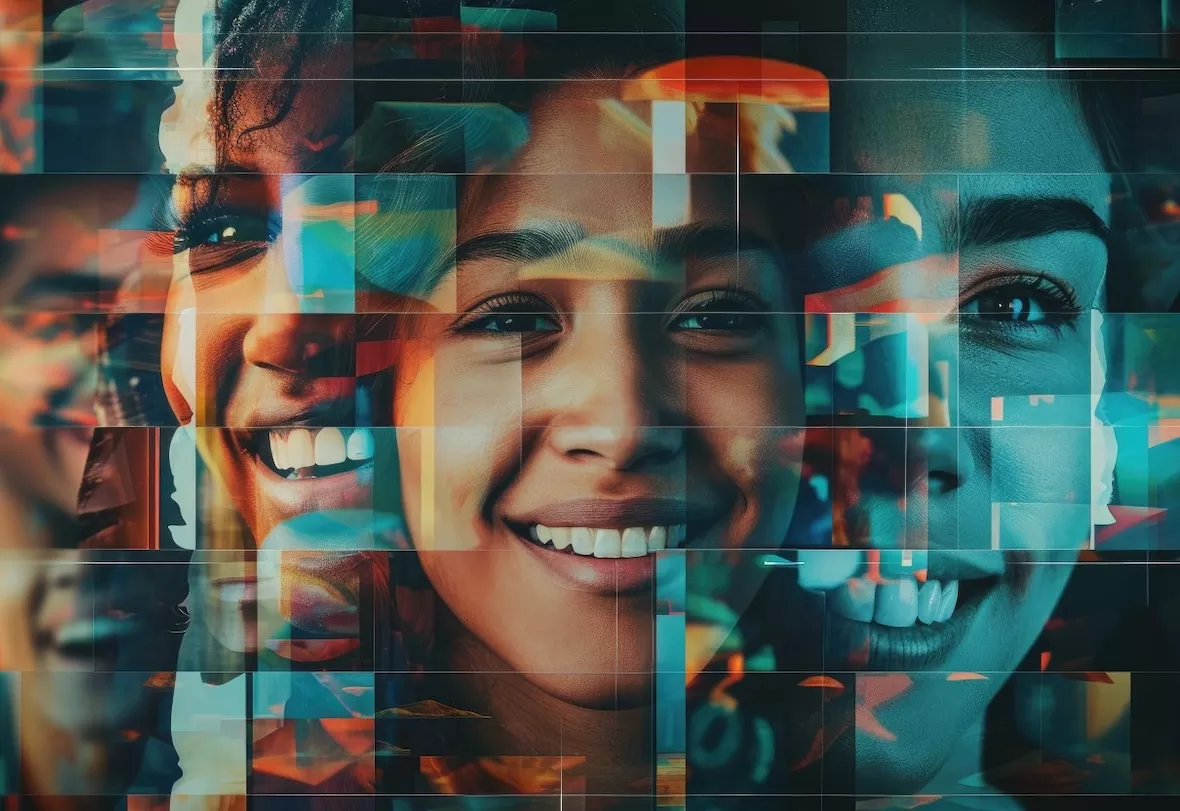
\includegraphics[keepaspectratio]{images/emotions.jpg}}

}

\caption{Emotion Recognition}

\end{figure}%

Ce projet permet de détecter les émotions humaines (joie, tristesse,
colère, etc.) en temps réel via la webcam.

📌 \textbf{Tech} : OpenCV, Deep Learning, CNN, Keras, Python.

\begin{center}\rule{0.5\linewidth}{0.5pt}\end{center}

\subsection{\texorpdfstring{📰
\href{https://github.com/dona-erick/VeritaAI}{Détection automatique de
Fake
News}}{📰 Détection automatique de Fake News}}\label{duxe9tection-automatique-de-fake-news}

\begin{figure}[H]

{\centering \pandocbounded{
\includegraphics[keepaspectratio]{images/fake-news.jpg}}

}

\caption{Fake News}

\end{figure}%

Développement d'un système intelligent capable d'identifier
automatiquement les fausses informations circulant en ligne.
Prétraitement, vectorisation, modélisation et suivi via MLflow.

📌 \textbf{Tech} : NLP, TF-IDF, SVM, RandomForest, MLflow

\begin{center}\rule{0.5\linewidth}{0.5pt}\end{center}

\subsection{🛒 API de Gestion de Ventes d'articles
téléphoniques}\label{api-de-gestion-de-ventes-darticles-tuxe9luxe9phoniques}

\begin{figure}[H]

{\centering \pandocbounded{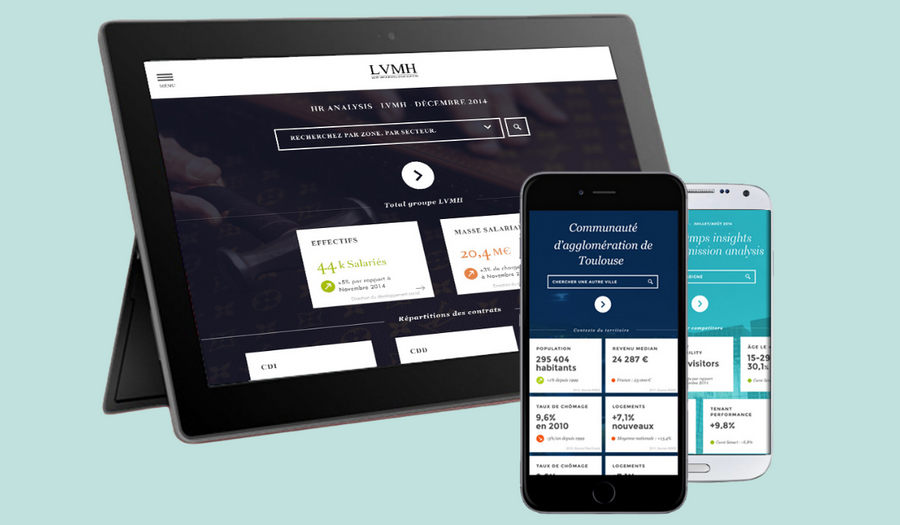
\includegraphics[keepaspectratio]{images/ventes.png}}

}

\caption{Ventes}

\end{figure}%

Développement des versions stables d'api intégrée à Flutter qui permet à
une boutique de ventes d'articles d'ajouter, modifier et de suivre en
temps réel ses ventes. Un dashboard dynamique est mit en plus pour
suivre de façon régulière et analytique ses articles .

📌 \textbf{Stack} : DjangoRestFramework, SQLite, Bootstrap,Python,
Flutter

🔒 \textbf{Code Source} :
\href{https://github.com/dona-eric/Gestion-des-ventes}{API}

\subsection{\texorpdfstring{\href{https://github.com/dona-eric/course-repo-coursera}{OnlineCourse(Coursera)}}{OnlineCourse(Coursera)}}\label{onlinecoursecoursera}

\begin{figure}[H]

{\centering \pandocbounded{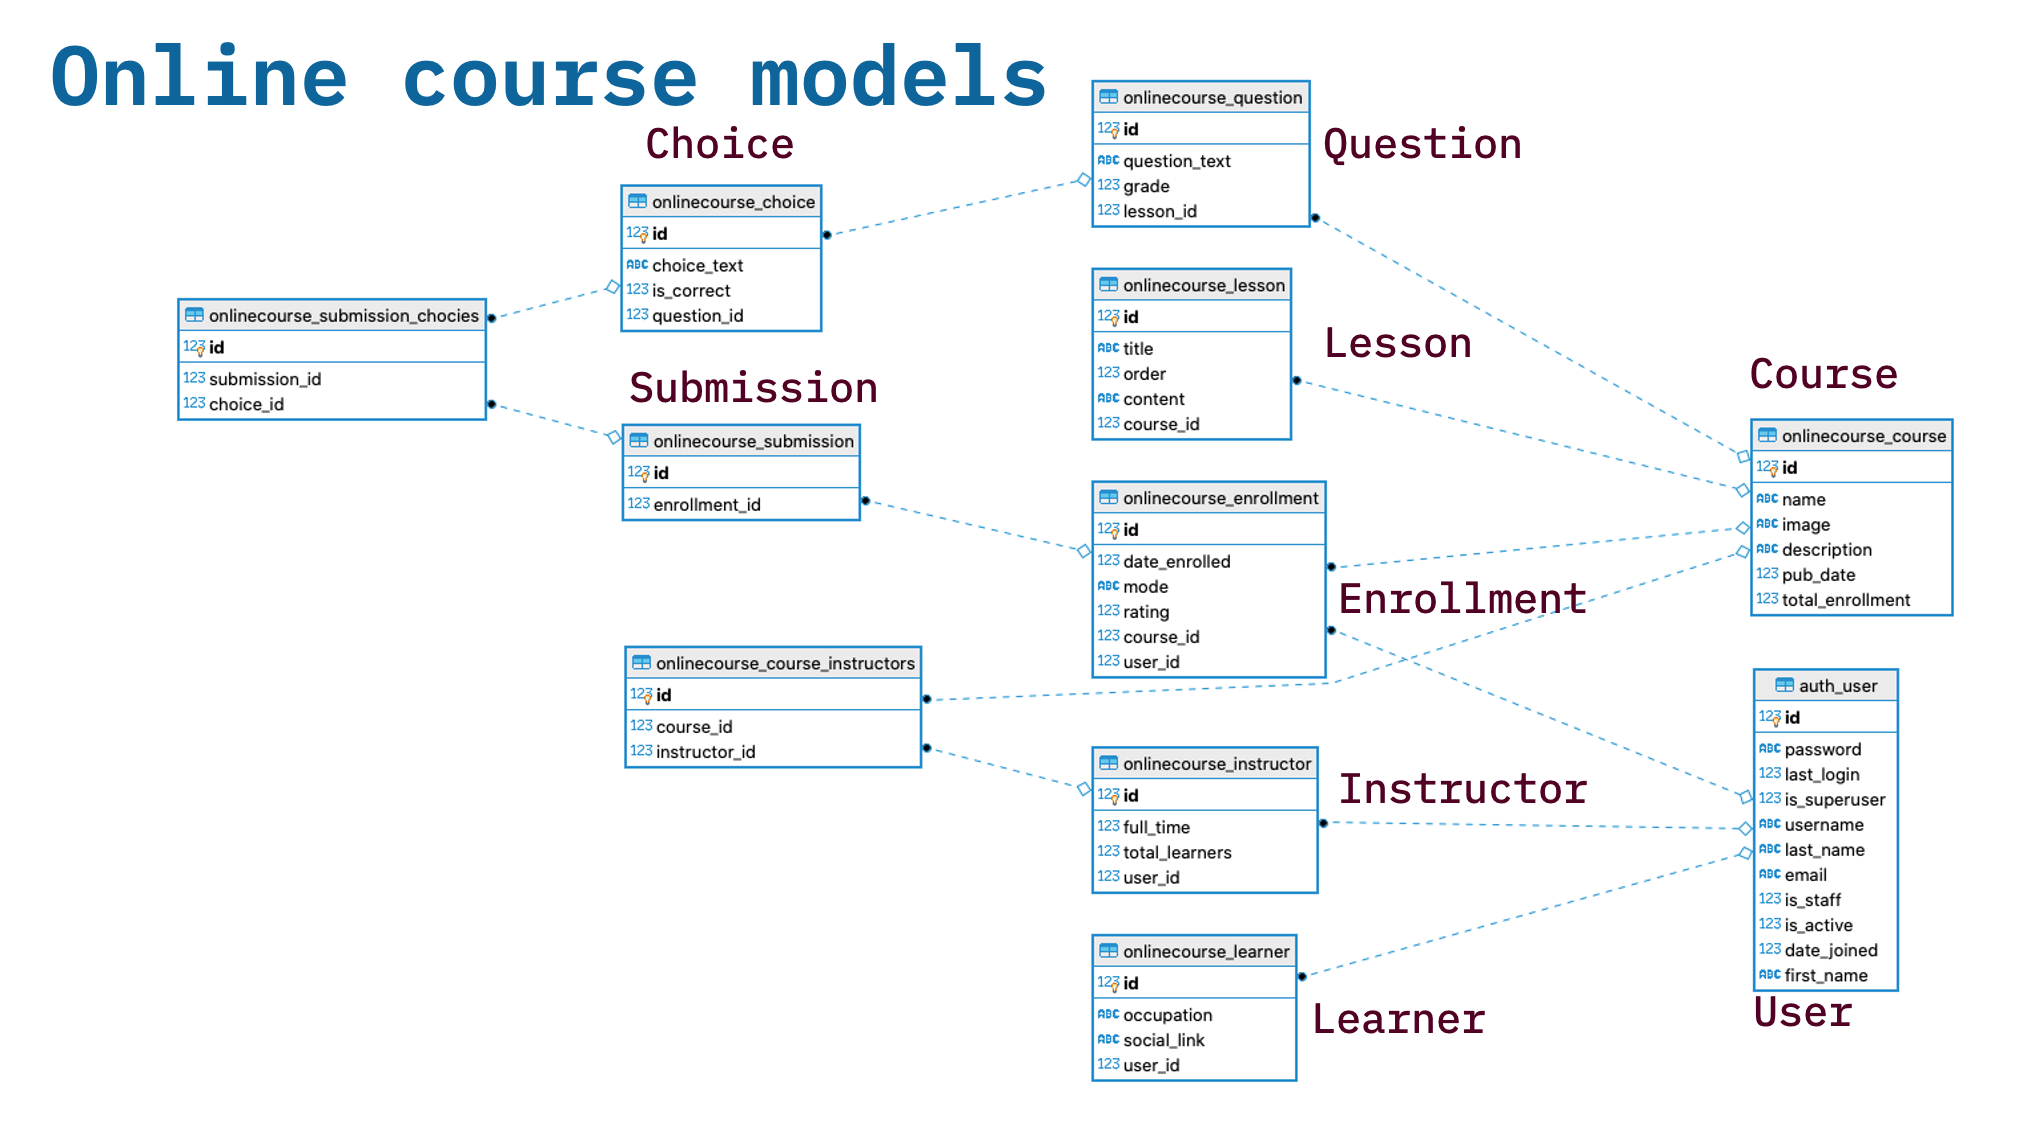
\includegraphics[keepaspectratio]{images/onlinecourse_app.png}}

}

\caption{coursera-architect}

\end{figure}%

OnlineCourse est une application qui a déjà été fournie dans ce
référentiel sur laquelle j'ai contribué en ajoutant une nouvelle
fonctionnalité d'évaluation. J'ai ainsi contribué au développement du
projet final sur Theia hébergé par IBM Developer Skills Network .

\begin{center}\rule{0.5\linewidth}{0.5pt}\end{center}

\subsection{🌐 Mon Portfolio}\label{mon-portfolio}

\begin{figure}[H]

{\centering \pandocbounded{\includegraphics[keepaspectratio]{images/portfolio.png}}

}

\caption{Portfolio}

\end{figure}%

Portfolio personnel développé avec \textbf{Quarto}, pour centraliser mes
projets, expériences, compétences et participations.

📌 \textbf{Tech} : Quarto, HTML, CSS, GitHub Pages 🔗
\href{https://github.com/dona-eric/dona-erick}{Voir le code source}

\begin{center}\rule{0.5\linewidth}{0.5pt}\end{center}

📬 Pour toute collaboration ou question technique, contactez-moi via
\href{https://www.linkedin.com/in/dona-erick/}{LinkedIn} ou directement
dans la section \textbf{Contact} du site.

\begin{quote}
✨ D'autres projets sont en cours de développement\ldots{} restez
connectés !
\end{quote}




\end{document}
